\chapter{適用例}\label{cha:Indication}
% 本章では、本研究で作成したモータ特性表自動生成ツールが正しく動作することを検証するため、以下の同じ能力である2種類のModelicaモデルのシミュレーション結果のcsvファイルを適用する。
本章では、本研究で作成したモータ特性表自動生成ツールが正しく動作することを確認する。
適用例として、ブラシ付きDCモータのModelicaモデルと、ブラシ付きDCモータのModelicaモデルをサブシステムとするモデル、の2つが出力するcsvファイルを適用例として用いる。
また、2つのモータの性能は同じである。
正しく動作しているか確認するために、以下の2つの点に着目する。
% 以下に示す2種類のModelicaモデルのシミュレーション結果のcsvファイルを適用例として用いる。
% 以下のモータは、性能は同じである。
% \begin{itemize}
%     \item ブラシ付きDCモータのModelicaモデル
%     \item ブラシ付きDCモータのModelicaモデルをサブシステムとするモデル
% \end{itemize}

% 2つのモデルのパラメータ設定を以下に示す。
% \begin{itemize}
%     \item 電源部品 ・・・ 9 V
%     \item 抵抗部品 ・・・ 1.78 $\Omega$
%     \item インダクタ部品 ・・・ 0.0000735 H
%     \item 起電力部品 ・・・ 0.010400000000000001 $mN \cdot m$
%     \item 慣性部品 ・・・ 0.00371135959 $\mathrm{kg\cdot m^2}$
% \end{itemize}
% 具体的には、以下の2つの項目を確認する。

\begin{enumerate}
    \item 生成したモータ特性表の各要素の値が、正しい値になっていること
    \item 2つのモデルから生成したモータ特性表の各要素が、同値になっていること
\end{enumerate}


\section{ブラシ付きDCモータのModelicaモデル}
ブラシ付きDCモータのModelicaモデルをOpenModelicaで実行し、生成されたcsvファイルを、モータ特性表自動生成ツールに適用する。適用例に用いるモデルを、図\ref{fig:tekiyou_tanntai}に、
図\ref{fig:tekiyou_tanntai}のシミュレーション結果であるcsvファイルからモータ特性表を作成する際に使用する要素を、図\ref{fig:tekiyou_csv}にそれぞれ示す。図\ref{fig:tekiyou_csv}の赤丸は最大値を、青い四角形は最大効率時の行を表す。
\begin{figure}[t]
	\centering
	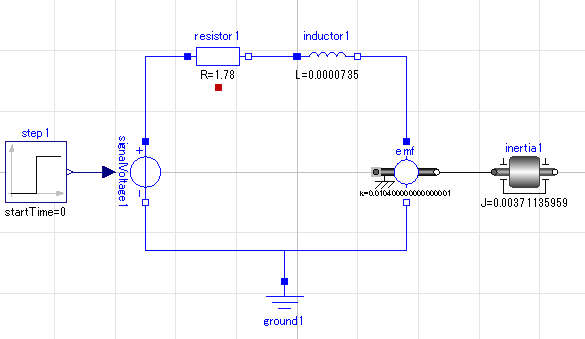
\includegraphics[width=10cm]{./Image/tekiyou_tanntai.png}
	\caption{適用するブラシ付きDCモータのModelicaモデル}
	\label{fig:tekiyou_tanntai}
\end{figure}
% \begin{figure}[t]
% 	\centering
% 	\fbox{
%     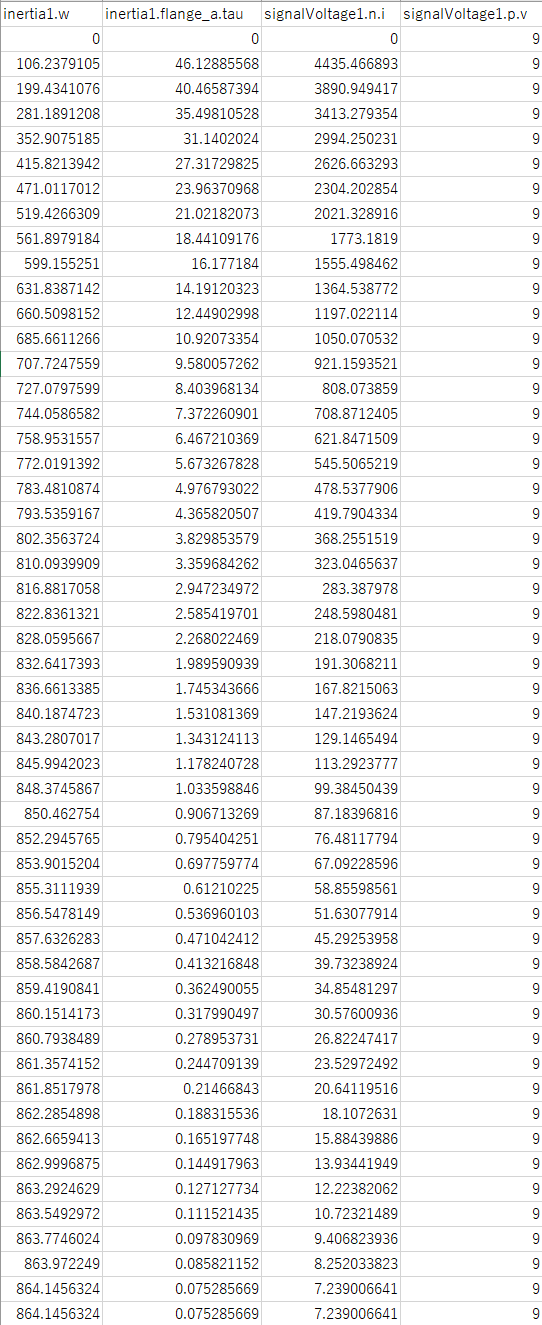
\includegraphics[width=9cm]{./Image/tekiyou_csv.png}
%     }
%     \caption{図\ref{fig:tekiyou_tanntai}のシミュレーション結果であるcsvファイルの一部}
% 	\label{fig:tekiyou_csv}
% \end{figure}
\begin{figure}[t]
	\centering
	\fbox{
    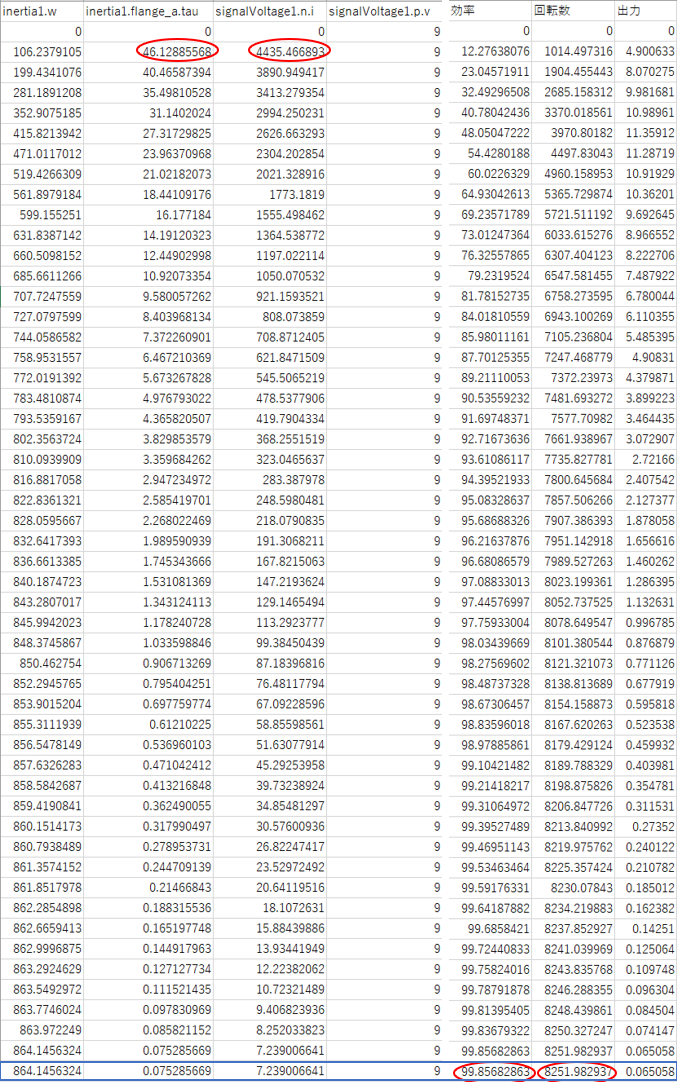
\includegraphics[width=13cm]{./Image/kakunin_saidai_mark.png}
    }
	\caption{図\ref{fig:tekiyou_tanntai}のシミュレーション結果であるcsvファイルの一部と効率と回転数}
	\label{fig:tekiyou_csv}
\end{figure}
図\ref{fig:tekiyou_csv}のcsvファイルをモータ特性表自動生成ツールに適用した結果、出力するモータ特性表を図\ref{fig:tekiyou_mortoku}に示す。
% \begin{figure}[t]
% 	\centering
% 	\fbox{
%     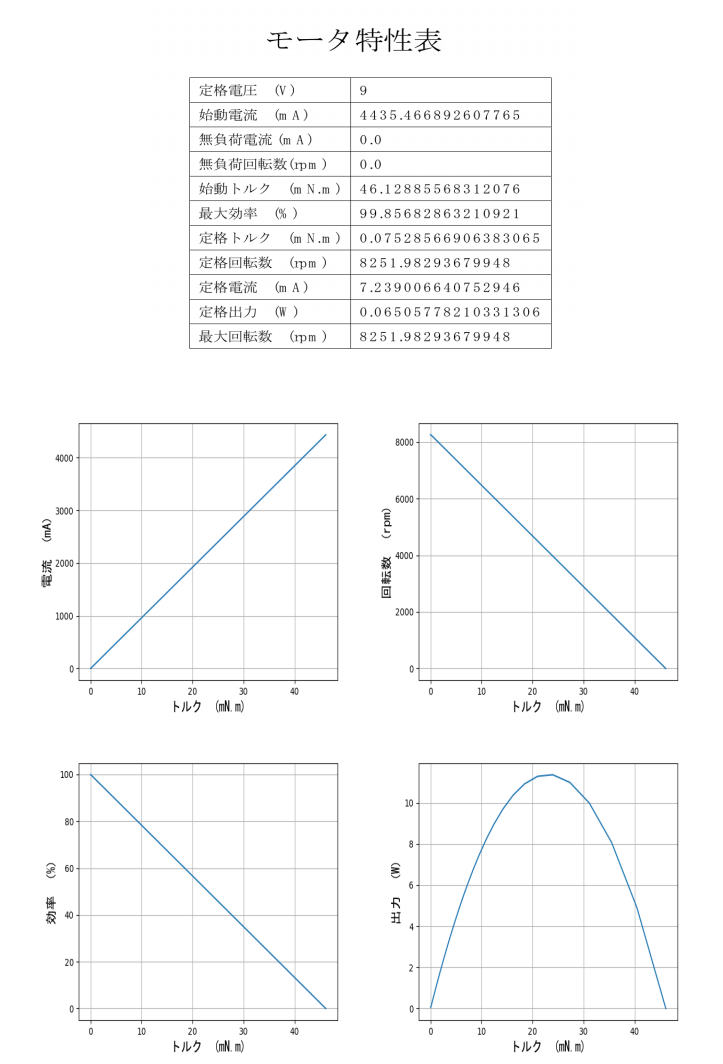
\includegraphics[width=14cm]{./Image/tekiyou_mortoku.png}
%     }
%     \caption{適用例で生成したモータ特性表}
% 	\label{fig:tekiyou_mortoku}
% \end{figure}
\begin{figure}[t]
	\centering
	\fbox{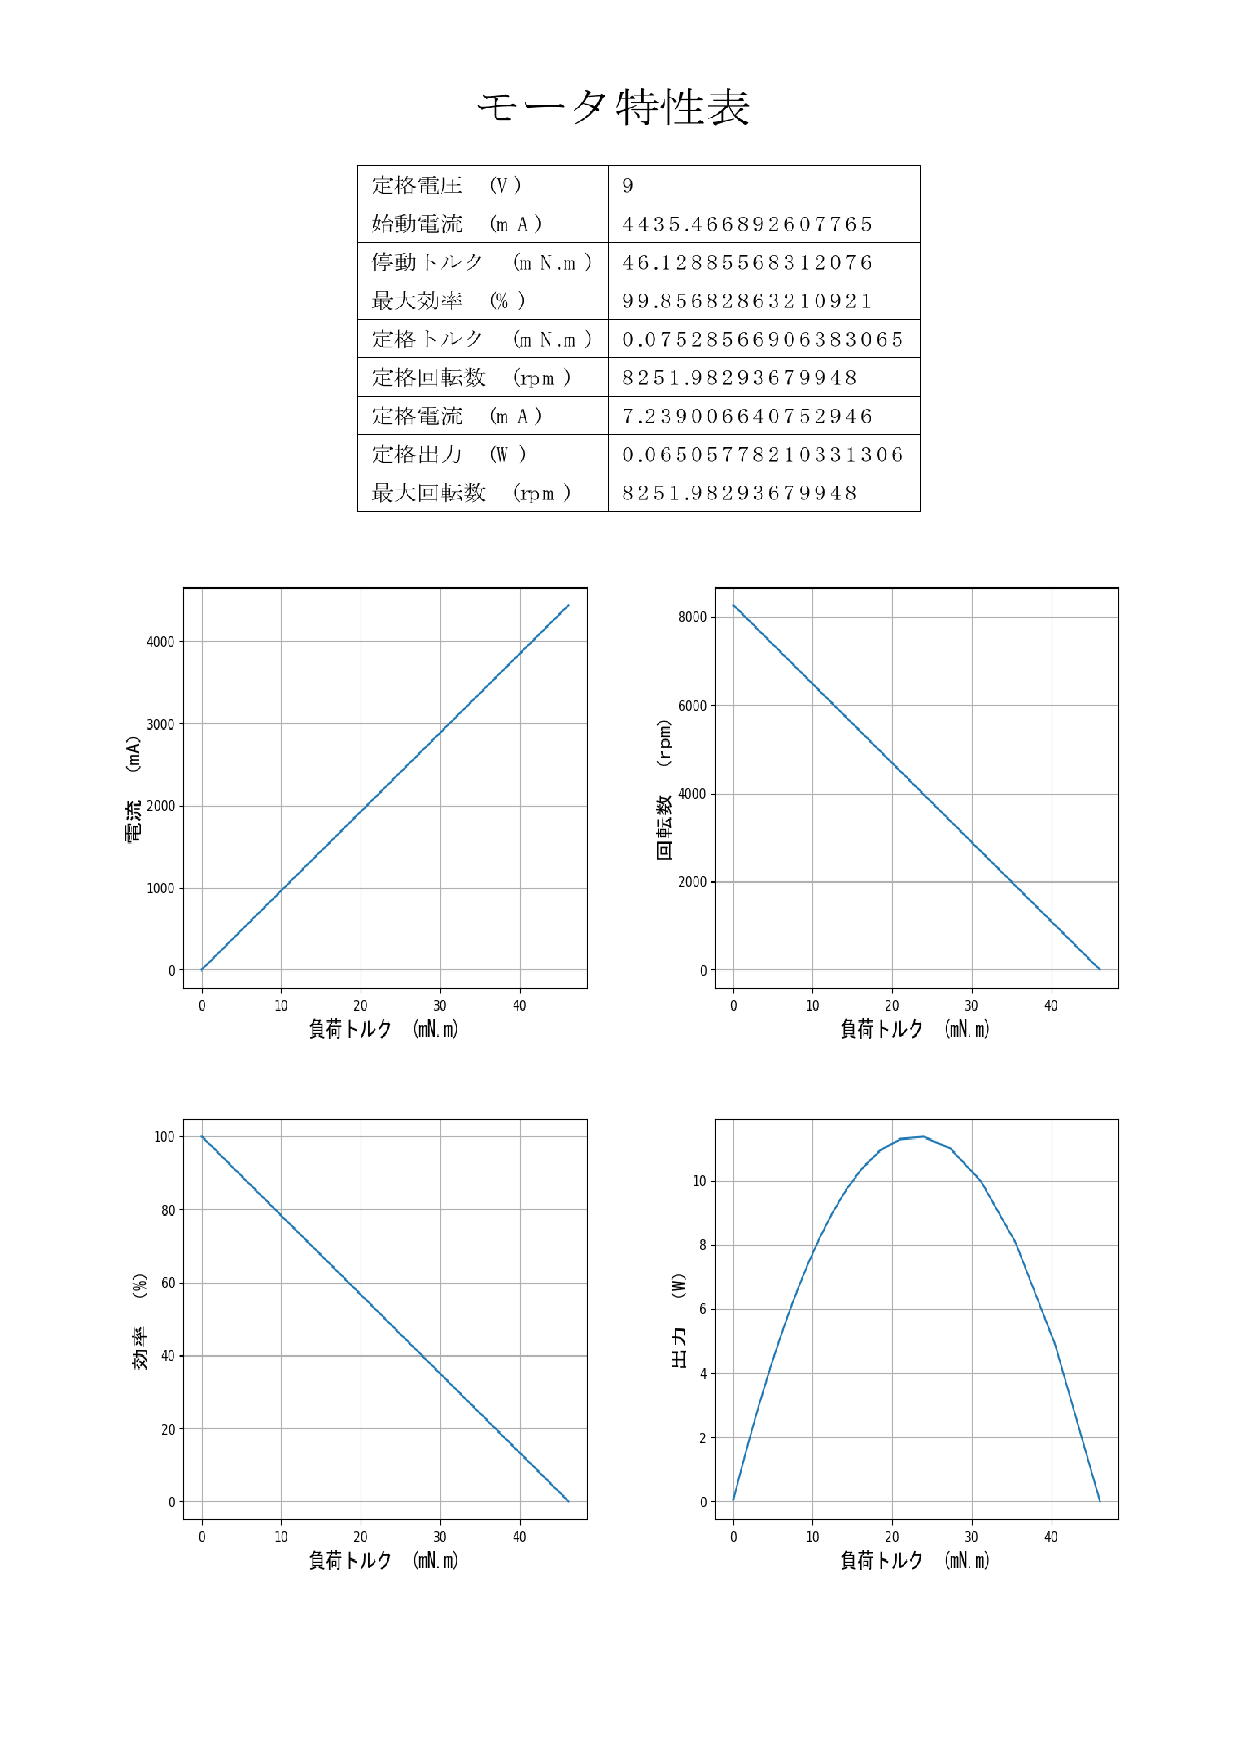
\includegraphics[width=16cm,pagebox=cropbox]{Image/characteristicTable_kakunin.pdf}}
	\caption{適用例で生成したモータ特性表}
	\label{fig:tekiyou_mortoku}
\end{figure}
\clearpage
\subsection{特性表の確認}
以下に、特性表で出力した各要素が正しく算出できているか確認する。%図\ref{fig:kakunin_csv}には、図\ref{fig:tekiyou_csv}から効率と回転数を算出したデータを示す。図中の赤丸は最大値を、青い四角形は最大効率時の行を表す。
% \begin{figure}[t]
% 	\centering
% 	\fbox{
%     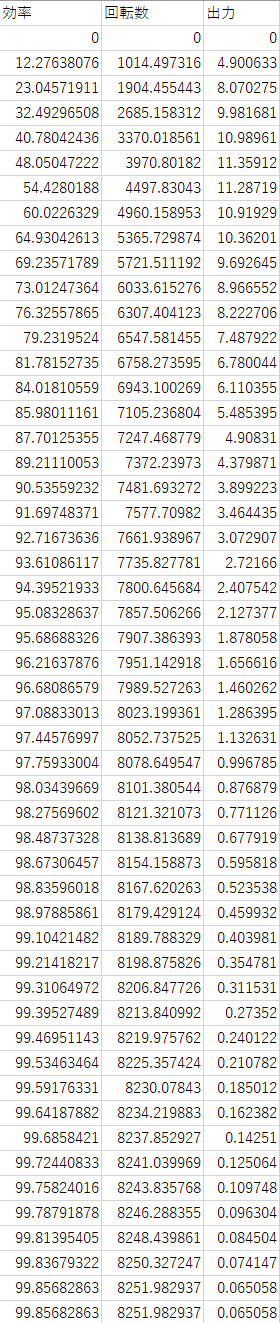
\includegraphics[width=3cm]{./Image/tekiyou_csv_kakunin.png}
%     }
%     \caption{図\ref{fig:tekiyou_csv}から効率と回転数を算出}
% 	\label{fig:kakunin_csv}
% \end{figure}

\subsubsection{定格電圧}
図\ref{fig:tekiyou_mortoku}の特性表にある定格電圧の値と、図\ref{fig:tekiyou_csv}のsignalVoltage1.p.vが持つ値の中で、先頭にある値が同値である。よって、正しく出力していることが確認できる。
\subsubsection{始動電流}
図\ref{fig:tekiyou_mortoku}の特性表にある始動電流の値と、図\ref{fig:tekiyou_csv}のsignalVoltage1.n.iが持つ値の中の最大値が同値である。よって、正しく出力していることが確認できる。
\subsubsection{停動トルク}
図\ref{fig:tekiyou_mortoku}の特性表にある停動トルクの値と、図\ref{fig:tekiyou_csv}のinertia1.flange\_a.tauが持つ値の中の最大値が同値である。よって、正しく出力していることが確認できる。
\subsubsection{最大効率}
図\ref{fig:tekiyou_mortoku}の特性表にある最大効率の値と、図\ref{fig:tekiyou_csv}の効率が持つ値の中の最大値が同値である。よって、正しく出力していることが確認できる。
\subsubsection{定格トルク}
図\ref{fig:tekiyou_mortoku}の特性表にある定格トルクの値と、図\ref{fig:tekiyou_csv}のinertia1.flange\_a.tauが持つ値の中の、最大効率を出した時の値が同値である。よって、正しく出力していることが確認できる。
\subsubsection{定格回転数}
図\ref{fig:tekiyou_mortoku}の特性表にある定格回転数の値と、図\ref{fig:tekiyou_csv}の回転数が持つ値の中の、最大効率を出した時の値が同値である。よって、正しく出力していることが確認できる。
\subsubsection{定格電流}
図\ref{fig:tekiyou_mortoku}の特性表にある定格電流と、図\ref{fig:tekiyou_csv}のsignalVoltage1.n.iが持つ値の中の、最大効率を出した時の値が同値である。よって、正しく出力していることが確認できる。
\subsubsection{定格出力}
% 出力は、\mbox{ トルク $(\mathrm{N \cdot m})$} $\times$ \mbox{角速度 $(\mathrm{rad/s})$} で算出することが可能である。
図\ref{fig:tekiyou_mortoku}の特性表にある定格出力と、図\ref{fig:tekiyou_csv}の出力が持つ値の中の、最大効率を出した時の値が同地である。よって、正しく出力していることが確認できる。
が同値である。よって、正しく出力していることが確認できる。
% 図\ref{fig:tekiyou_mortoku}の特性表にある出力と、図\ref{fig:tekiyou_csv}の最大効率時のinertia1.flange\_a.tauが持つ値と、inertia1.flange\_a.wが持つ値を(\ref{siki:speed})式に適用した結果が同値である。
% よって、正しく出力していることが確認できる。
\subsubsection{最大回転数}
図\ref{fig:tekiyou_mortoku}の特性表にある最大回転数と、図\ref{fig:tekiyou_csv}の回転数が持つ値の中の最大値が同値である。よって、正しく出力していることが確認できる。
\subsection{特性グラフの確認}
以下に、特性グラフが正しく生成できているか確認する。

\subsubsection{「負荷トルク $\times$ 電流」グラフ}
図\ref{fig:tekiyou_csv}のinertia1.flange\_a.tauの持つ値と、signalVoltage1.n.iが持つ値を確認できるので、正しく生成していることが確認できる。
\subsubsection{「負荷トルク $\times$ 回転数」グラフ}
図\ref{fig:tekiyou_csv}のinertia1.flange\_a.tauの持つ値と、回転数が持つ値を確認できるので、正しく生成していることが確認できる。
\subsubsection{「負荷トルク $\times$ 効率」グラフ}
図\ref{fig:tekiyou_csv}のinertia1.flange\_a.tauの持つ値と、効率が持つ値を確認できるので、正しく生成していることが確認できる。
\subsubsection{「負荷トルク $\times$ 出力」グラフ}
図\ref{fig:tekiyou_csv}のinertia1.flange\_a.tauの持つ値と、出力が持つ値を確認できるので、正しく生成していることが確認できる。

したがって、生成したモータ特性表の各要素の値が、正しい値になっていることを確認できる。

\section{ブラシ付きDCモータのModelicaモデルをサブシステムとするモデル}
今回適用するブラシ付きDCモータのModelicaモデルをサブシステムとするモデルは、図\ref{fig:tekiyou_tanntai}のモデルと同じ性能になるよう設計しており、どちらのモータ特性表も同じ内容になっていることを確認する。

今回適用するブラシ付きDCモータのModelicaモデルをサブシステムとするモデルを図\ref{fig:tekiyou_sub}に、生成したモータ特性表を図\ref{fig:sub_mortoku}にそれぞれ示す。

\begin{figure}[t]
	\centering
	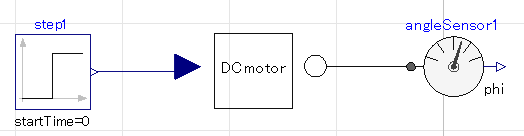
\includegraphics[width=10cm]{./Image/tekiyou_sub.png}
	\caption{適用するブラシ付きDCモータのModelicaモデルをサブシステムとするモデル}
	\label{fig:tekiyou_sub}
\end{figure}

\begin{figure}[t]
	\centering
	\fbox{
	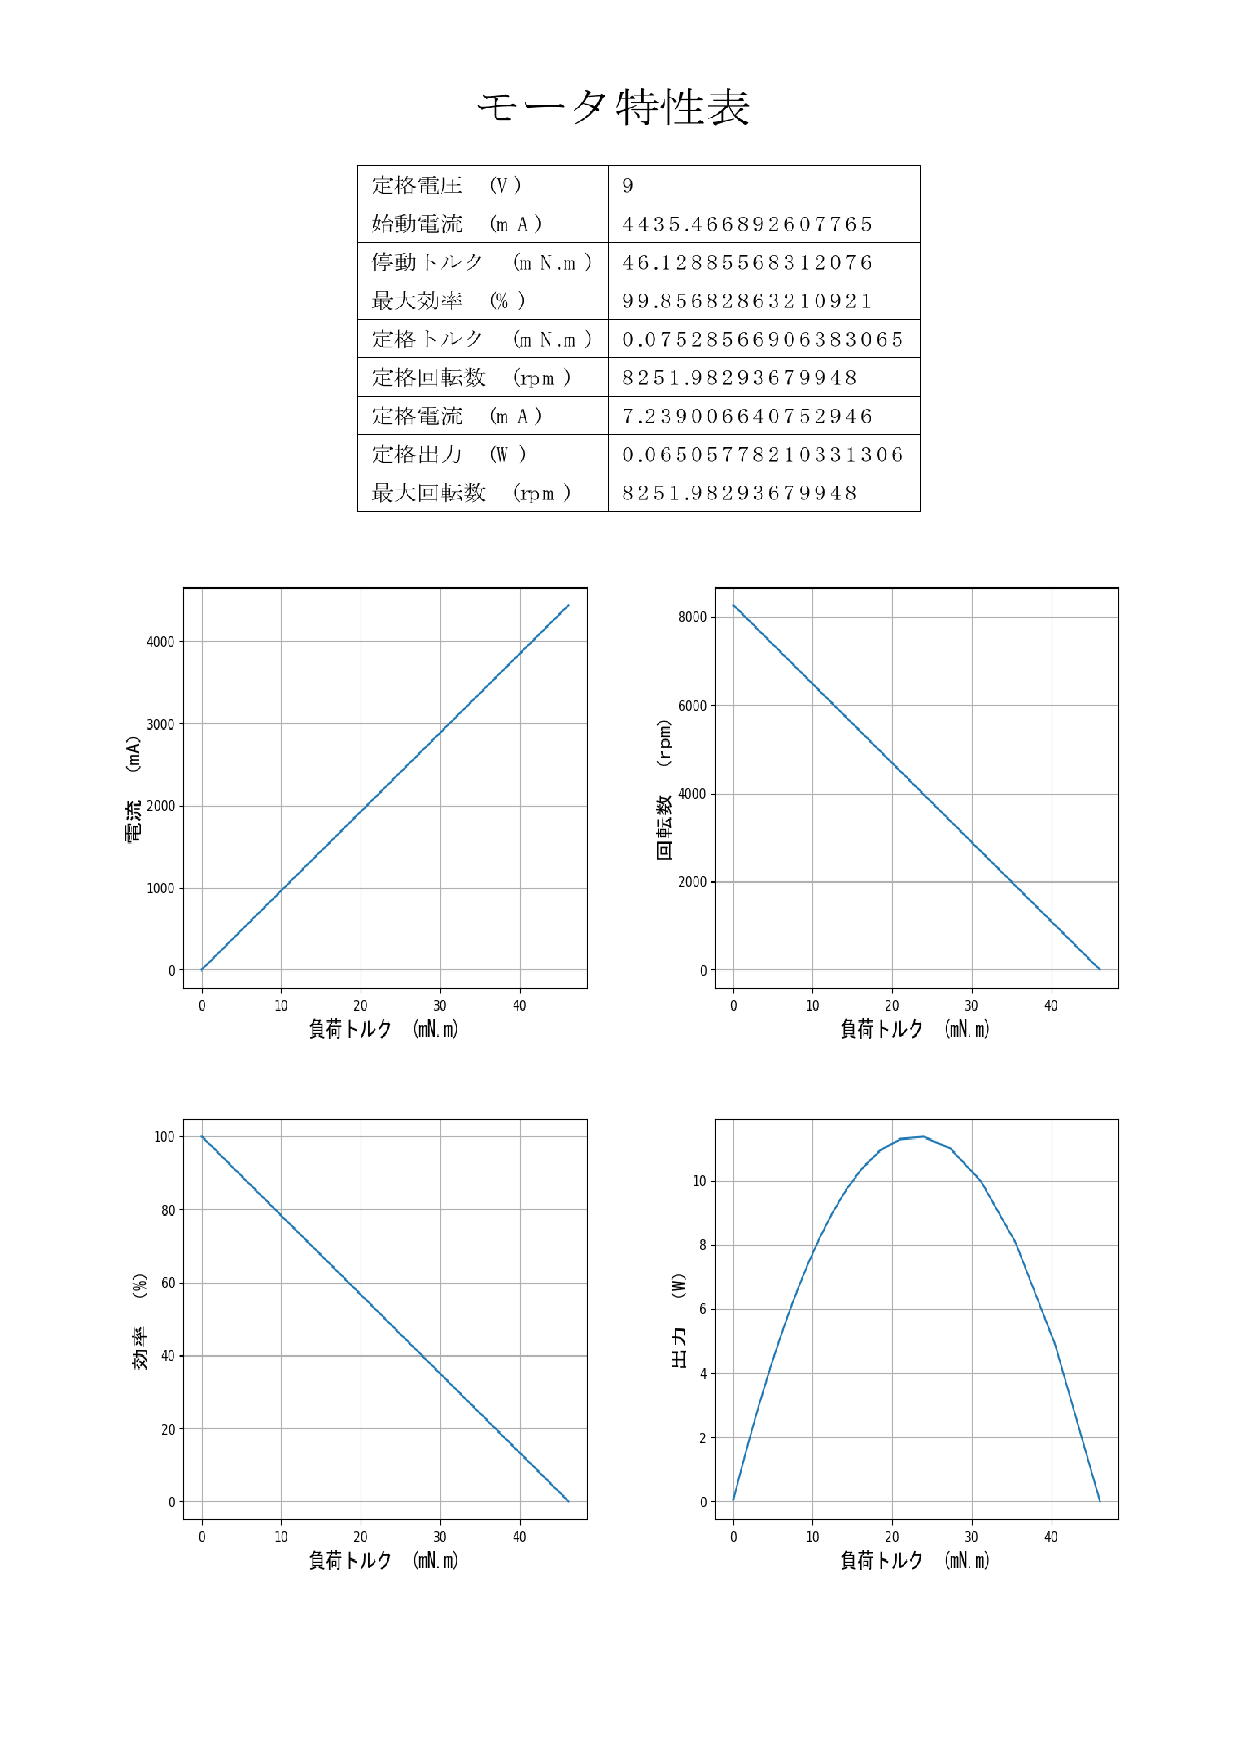
\includegraphics[width=16cm,pagebox=cropbox]{Image/characteristicTable_kakunin.pdf}
	}
	\caption{図\ref{fig:tekiyou_sub}のモータ特性表}
	\label{fig:sub_mortoku}
\end{figure}

図\ref{fig:tekiyou_mortoku}と図\ref{fig:sub_mortoku}の内容が同じであるため、2つのモデルから生成したモータ特性表の各要素が、同値になっていることが確認できる。

よって、モータ特性表自動生成ツールは、「ブラシ付きDCモータのModelicaモデル」と「ブラシ付きDCモータのModelicaモデルをサブシステムとするモデル」に対応していることが確認できる。